\section{Trabalhos Relacionados}
\paragraph{}A análise de praias e mares através de imagens não é algo novo. O uso de câmeras oferece uma grande vantagem em relação a outros tipos de sensores, como descrito por Holland\cite{Holland97}, "Técnicas de vídeo são particularmente atraentes na documentação de processos oceanográficos próximos a costa uma vez que a localização subaérea do instrumento (distante da superfície do oceano) alivia algumas das dificuldades associadas com intrumentação \textit{in situ}, como a perturbação de correntes, bioincrustação e deteriorização dos sensores em condições adversas de ondas". Entretanto, não existem muitos projetos diretamente ligados à análise de ondas marítimas utilizando processamento de imagem. O desenvolvimento mais notório nessa área é feito na Griffith University, Austrália, onde foram desenvolvidos alguns projetos e técnicas de monitoramento de praias que serão descritos a seguir. 
%Griffith05
\paragraph{}Browne \textit{et al.} \cite{Griffith05} descrevem um sistema inteligente que monitora e prediz as condições de uma praia para banho. O objetivo desse sistema é, em caso de perigo, alertar aos banhistas e às autoridades sobre o estado da praia em tempo real. O sistema obtém dados da praia de duas fontes: de câmeras posicionadas \textit{in loco} e de servidores do \textit{Bureau of Meteorology} australiano.
As imagens obtidas são pré-processadas, extraindo dados como tamanho e frêquencia das ondas e a localização da arrebentação. Dos servidores são obtidos dados em tempo real sobre as marés, vento e \textit{swell}, que são as ondas formadas por tempestades e ventos distantes, e não por vento local. Uma vez obtidos os dados, o sistema alimenta uma rede neural treinada que determina se a praia é segura para banho.
%Griffith10
\paragraph{}Outro sistema estudado é chamado de \textit{WavePack} \cite{Griffith10}, descrito nesse artigo apenas de forma não-técnica. Esse sistema tem como objetivo apenas medir a altura, frequência e localização do momento que uma onda quebra, utilizando câmeras montadas em pontos baixos, dez metros acima da praia. O sistema é descrito em quatro etapas: obtenção das imagens, conversão do \textit{stream} de vídeo em \textit{timestack}, análise do \textit{timestack}, apresentação dos resultados. O artigo ainda compara os resultados obtidos com outras fontes de dados de ondas marítimas, e comprova que o sistema produz dados confiáveis. 
%Griffith11 e Griffith14
\paragraph{}O algoritmo implementado no sistema \textit{WavePack} é descrito em um artigo \cite{Griffith11} posterior. Esse artigo descreve o método de: 1) identificar a arrebentação, e 2) identificar cada onda individual na arrebentação e calcular a sua altura em pixels, filtrando a perturbação de objetos indesejados na imagem (como barcos e pessoas). Em seguida, é discutida e apresentada a relação entre a altura de uma onda medida em pixels e a sua altura no mundo real, em metros. Por último, apresenta-se os resultados obtidos, novamente comparados com outros métodos já existentes. Esse método é também apresentado também é apresentado em um artigo \cite{Griffith14} mais recente. Esse artigo descreve com maiores detalhes o pré-processamento que ocorre no \textit{timestack}, e a relação entre a altura da onda encontrada em pixels e a altura em metros no mundo real.
\paragraph{}Essas pesquisas serviram de grande inspiração para o desenvolvimento deste projeto, mostrando que ele é factível. Os resultados desses projetos servirão como parâmetro de validação dos aqui resultados encontrados.
\paragraph{}No Brasil não é conhecido algum sistema de monitoramento de praias automatizado. No Rio de Janeiro o site RicoSurf\cite{Rico17} provém um monitoramento manual de algumas praias locais e de cidades próximas, se expandindo até Guarapari, ES. O monitoramento é feito através de boletins disponíveis no site, que normalmente são feitos uma ou duas vezes ao dia por uma pessoa que vai até a praia e reporta a condição encontrada. Este método é pouco prático se aplicado em grande escala, é subjetivo e demanda uma quantidade cada vez maior de repórteres para analisar cada praia. 
\section{Processamento de Vídeo e Imagens}
\paragraph{}Processamento de Imagem é uma sequência de operações realizadas em uma ou mais imagens de entrada, resultado em uma imagem de saída ou características extraídas das imagens de entrada. Uma imagem, conforme definido por Rafael Gonzalez \cite{Gonzalez92} é: "[...] uma função bidimensional \(f(x,y)\), onde \(x\) e \(y\) são coordenadas espaciais (plano), e a amplitude de \(f\) de qualquer par de coordenadas \((x,y)\) é chamada de intensidade ou nivel de cinza da imagem naquele ponto.".
\paragraph{}Neste projeto, como em outras aplicações de oceanografia \cite{Jahne02} \cite{Holland97}, imagens estáticas do objeto de estudo são pouco produtivas para extrair informações. Por isso, uma solução encontrada foi capturar e trabalhar com um vídeo da arrebentação de uma praia, ao invés de usar apenas fotografias. 
\paragraph{}Um vídeo é definido como uma sequência temporal de imagens. De forma análoga a imagem, um vídeo pode ser descrito como uma função tridimensional \(g(x,y,t)\), onde \(x\) e \(y\) são coordenadas espaciais, como em uma imagem, e \(t\) é uma coordenada temporal. A amplitude \(g\) é a intensidade ou nível de cinza do ponto \((x,y)\) no instante de tempo \(t\).
\paragraph{}A principal vantagem de utilizar um vídeo é eliminar o problema de identificar qual é o melhor momento para analisar a onda fotografada. Utilizando uma sequência de imagens, é mais fácil de determinar qual foi o momento em que a onda estava maior, e ai sim realizar a medição de sua altura. Será demonstrado adiante que o timestack também ajuda a tornar as imagens analisadas mais uniformes, criando regiões bem definidas para segmentaçao. 
\section{Identificação de objetos} %features ?
\paragraph{}Para extrair os dados desejados de uma imagem, é necessário separar o que é o objeto de estudo -- no caso específico deste projeto, uma onda do mar -- do restante da imagem. Isto é, através de transformações na imagem original deseja-se identificar o que é o primeiro plano e o plano de fundo. Este processo de extração de objetos ou planos de uma imagem é chamado na literatura de segmentação \cite{Gonzalez92}.
\paragraph{}Antes de aplicar as técnicas de segmentação, precisa-se melhorar a imagem. O processo de aprimoramento de imagens, segundo Rafael Gonzalez \cite{Gonzalez92}, é fundamental para torná-la adequada para a aplicação desejada. O aprimoramento permite realçar alguma característica de interesse da imagem, enquanto minimiza a presença de outras características não relevantes.
%\paragraph{}O aprimoramento pode ser realizado em dois domínios: domínio espacial e domínio da frequência.
\paragraph{}Os métodos de aprimoramento de imagens são classificados em dois domínios: domínio espacial e domínio da frequência. 
O aprimoramento no domínio espacial trabalha com os próprios pixels de uma imagem, e podem ser representados pela expressão: \(g(x,y) = T[f(x,y)]\), onde \( g(x,y) \) é a imagem transformada, \( f(x,y) \) é a imagem original e \( T[ \ \cdot\  ] \) é a transformação que será aplicada na imagem original.
%TODO: Falar sobre métodos no domínio da frequência
\paragraph{}Alguns métodos de aprimoramento de imagens serão utilizados nesse projeto: transformações em níveis de cinza, filtros de nitidez (\textit{sharpening}), filtros de suavização (\textit{blur}), filtros de detecção de bordas. Esses métodos são importantes para melhorar o contraste entre as regiões da imagem analisada e reduzir o ruído, facilitando assim o processo de segmentação que será realizado posteriormente.
\paragraph{}As transformações em níveis de cinza englobam métodos que alteram o contraste de uma imagem. Em geral, são métodos onde cada pixel \((x,y)\) da saída depende apenas do pixel correspondente da entrada, ou seja, não é influenciado pelos seus vizinhos. O principal método que será utilizado nesse projeto é o de \textit{thresholding}, onde a transformação aplicada na entrada é da forma: 
\[
T[f(x,y)] =
\begin{cases}
        f(x,y), & \text{se } f(x,y) > C\\
        0, & \text{se } f(x,y) < C
\end{cases}
\] 
\noindent{}Onde C é uma constante escolhida arbitrariamente. A utilidade dessa função é facilitar a definição das regiões da imagem, quais fazem parte do céu, do mar e da arrebentação.
\paragraph{}Os filtros de suavização, também conhecidos como filtros de \textit{blur} são importantes para reduzir o nível de ruído na imagem. Outra função importante para esse projeto é homogeneizar as regiões da imagem, isto é, eliminar, ou pelo menos reduzir, pontos mais claros em regiões escuras, ou pontos escuros em regiões claros. Dessa forma, os métodos de \textit{thresholding} são mais efetivos.
\paragraph{}Neste projeto o filtro de suavização utilizado é o filtro passa-baixas gaussiano. Este filtro, como definido em \cite{Gonzalez92}, possui a seguinte forma:
\[
H(u,v) = e^{-D^{2}(u,v)/2D^{2}_{0}}
\]
\noindent{}\(D(u,v)\) é definido como a distância da origem da transformada de Fourier, e \(D^{2}_{0}\) é definido como \(\sigma^{2}\), ou a variância da curva gaussiana.
\paragraph{}Segundo Bernd Jähne \cite{Jahne02}, um filtro de suavização deve atender algumas propriedades especificas para ser aplicável a identificação de objetos e extração de dados de uma imagem. As propriedades são:
\begin{enumerate}
\item Desvio de fase zero, isto é, o filtro não deve causar desvio na fase da imagem a fim de não alterar a posição dos objetos na mesma.
\item Preservação da média, isto é, a soma de todos os fatores da máscara no domínio espacial deve ser igual a 1.
\item Monotonicidade, isto é, a função de transferência do filtro de suavização deve decrescer monotonicamente.
\item Equidade, isto é, a função de transferência deve ser isotrópica, a fim de não privilegiar nenhuma direção na imagem.
\end{enumerate}
\paragraph{}Por último, uma classe de métodos de suma importância são os métodos de nitidez, ou \textit{sharpening}. A função desses métodos é aumentar o contraste da imagem na fronteira de regiões, isto é, onde ocorre uma descontinuidade de pixels. O método utilizado neste projeto é o método Laplaciano. Segundo Gonzalez \cite{Gonzalez92}, o Laplaciano de uma imagem \(f(x,y)\) é definido por:
\[
        \nabla^{2}f = \frac{\partial^{2}f}{\partial x^{2}} + \frac{\partial^{2}f}{\partial y^{2}}
\]
\paragraph{}As derivadas parciais da equação acima podem ser escritas na forma discreta:
\[
        \frac{\partial^{2}f}{\partial x^{2}} = f(x + 1,y) + f(x - 1,y) - 2f(x,y)
\]
\noindent{}e
\[
        \frac{\partial^{2}f}{\partial y^{2}} = f(x,y + 1) + f(x,y - 1) - 2f(x,y)
\]
\noindent{}\newline{}Dessa forma, o Laplaciano bidimensional discreto é dado por:
\[ 
        \nabla^{2}f = f(x + 1,y) + f(x - 1,y) + f(x,y + 1) + f(x,y - 1) - 4f(x,y) 
\]
\paragraph{}A aplicação de um operador Laplaciano em uma imagem resulta em suas apenas as suas descontinuidades. Pela definição do Laplaciano discreto, é fácil perceber que regiões com valores intensidades próximas se anulam, resultado em um Laplaciando próximo de zero, enquanto regiões com descontinuidade a diferença de intensidade se reforça. Para recuperar as regiões anuladas pelo Laplaciano e enfim aplicar o efeito de \textit{sharpening} na imagem, basta somar o resultado do Laplaciano com a imagem original:
\[ 
        g(x,y) = f(x,y) + \nabla^{2}f(x,y) 
\] 
\noindent{}Onde \(g(x,y)\) é a imagem de saída e \(f(x,y)\) é a imagem de entrada.


\subsection{Métodos de Segmentação de Imagens}

\paragraph{}Segmentação é definido como um processo que, a partir de uma imagem de entrada, a subdivide em objetos ou nas suas regiões constituintes. O nível de subdivisões que serão obtidas depende de cada aplicação, e segundo Gonzalez: "A segmentação deve parar quando os objetos de interesse em uma aplicação estejam isolados" \cite{Gonzalez92}. Além diso, Gonzalez continua: "A segmentação de imagens não-triviais é uma das tarefas mais difíceis em processamento de imagem" \cite{Gonzalez92}.
\paragraph{}O primeiro passo para realizar a segmentação é aplicar um método de detecção de bordas. O método escolhido para esse projeto é o método de Canny \cite{Canny86}, que é hoje o método mais eficaz de detecção de bordas \cite{Juneja09}. Esse método basea-se em criar um modelo matemático para uma borda e definir três restrições que o modelo deve atender, e então utilizar um método numérico para otimizar o modelo. As restrições definidas por Canny \cite{Canny86} são:
\begin{enumerate}
\item Boa detecção. Deve haver uma baixa probabilidade de detectar bordas inexistentes ou não detectar bordas existentes.
\item Boa localização. A localização das bordas detectadas deve estar próxima da localização das bordas reais.
\item Resposta única para cada borda. Uma borda não pode ser detectada multiplas vezes.
\end{enumerate}
\noindent{}Outro método de detecção de bordas considerado foi o método de Sobel \cite{Gonzalez92}, que é utilizado em \cite{Griffith11} para evidenciar bordas verticais. Uma diferença importante entre os dois método é que o método de Sobel atua em cada direção separadamente, podendo-se somar o resultado de cada direção para obter uma resposta unificada, enquanto o método de Canny atua em todas as direções simultaneamente. Devido a maior presença de ruído nas imagens capturadas, o método de Canny mostrou-se mais eficaz em eliminar o ruído e detectar apenas as bordas desejadas.
\paragraph{}O segundo passo do processo de segmentação é aplicar um método de extração de regiões. Este projeto utiliza o método de watershed \cite{Gonzalez92} para tal tarefa. O algoritmo de watershed baseia-se na idéia de enxergar a imagem em três dimensões como um vales que serão "inundados", sendo \(x\) e \(y\) coordenadas espaciais e a intensidade de cada pixel \(g(x,y)\) a "altura" de cada ponto neste vale. Os pontos de mínimo locais, ou seja, os pontos onde \(g(x,y)\) é mínimo localmente, consideramos este um ponto mais baixo de um vale, e a região ao redor que será segmentada sua zona de influência. A partir dos pontos de mínimo locais inunda-se a imagem, preenchendo-a com valores gradativamente maiores de intensidade de pixel em sua zona de influência, como seria o nível de água subindo em uma inundação. Eventualmente, a inundação da zona de influência de um ponto mínimo local irá "vazar" para a zona de influência de outro ponto mínimo local. Quando isso ocorre, constrói-se uma "barragem" com largura de um pixel entre as duas zonas de influência, para evitar o vazamento. Quando o nível de inundação atinge o ponto máximo da imagem, isto é, o valor máximo de \(g(x,y)\), o algoritmo de watershed é interrompido. As regiões segmentadas serão definidas pelas "barragens" formadas durante a execução do algoritmo. Na forma descrita acima, o algoritmo de watershed pode levar a segmentação de mais regiões que se desejava originalmente. Isso é corrigido através do uso de marcadores, indicadores de quais são os pontos de mínimo local que serão utilizados pelo algoritmo.

\section{Modelo Geométrico de Câmeras}

\paragraph{}Todos os métodos descritos anteriormente foram apresentados com o intuito de aplicá-los no cálculo da altura de uma onda em pixels. Para obter a altura em metros, precisa-se de um modelo matemático que relacione as duas medidas. O modelo mais simples de uma câmera é o modelo furo-de-agulha. Segundo Fusiello \cite{Fusiello}, o modelo é descrito pelo seu centro ótico \(C\) e o plano da imagem. A distância entre \(C\) e o centro do plano da imagem, é chamado de distância focal \(f\). O eixo perpendicular ao plano da imagem que passa pelo centro ótico é chamado de eixo principal.
%TODO: adicionar aqui imagem de \cite{Fusiello} 
\begin{figure}[h]
\begin{center}
  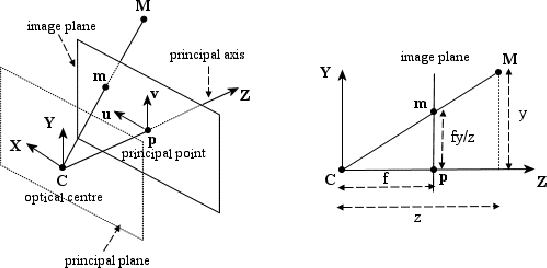
\includegraphics[scale=0.7]{pin_hole_camera.png}
  \caption[\small{Modelo de Câmera Furo-de-Agulha. Fonte: School of Informatics/University of Edinburgh \cite{Fusiello}.}]{\label{FigFusiello} \small{Modelo de Câmera Furo-de-Agulha. Fonte: School of Informatics/University of Edinburgh \cite{Fusiello}.}}
\end{center}
\end{figure}
\noindent{}Este modelo apresenta uma forma simples de calcular a relação entre a altura aparente de um objeto em uma imagem e a sua altura real, dependendo apenas da distância focal da câmera e da distância real do objeto. Esta relação é:
\[
        h_{real} = z * h_{aparente} / f
\]
\noindent{}onde \(z\) é a distância real do objeto, \(f\) é a distância focal, \(h_{real} e h_{aparente}\) são, respectivamente, a altura real e a altura aparente.
\section{Modelo Geométrico de Uma Praia}
\paragraph{}Browne \textit{et al.} \cite{Griffith14} descreve um modelo geométrico simplificado de uma praia, onde temos uma relação direta entre a altura em pixels de uma onda e a sua altura real. Para isso, são necessários três parâmetros de montagem da câmera: o ângulo da câmera em relação ao ponto de montagem (\(\phi_{t}\)), o ângulo de \textit{zoom} da câmera (\(\phi_{z}\)) e a altura da câmera em relação ao nível do mar (\(h_{c}\)).
\begin{figure}[h]
\begin{center}
  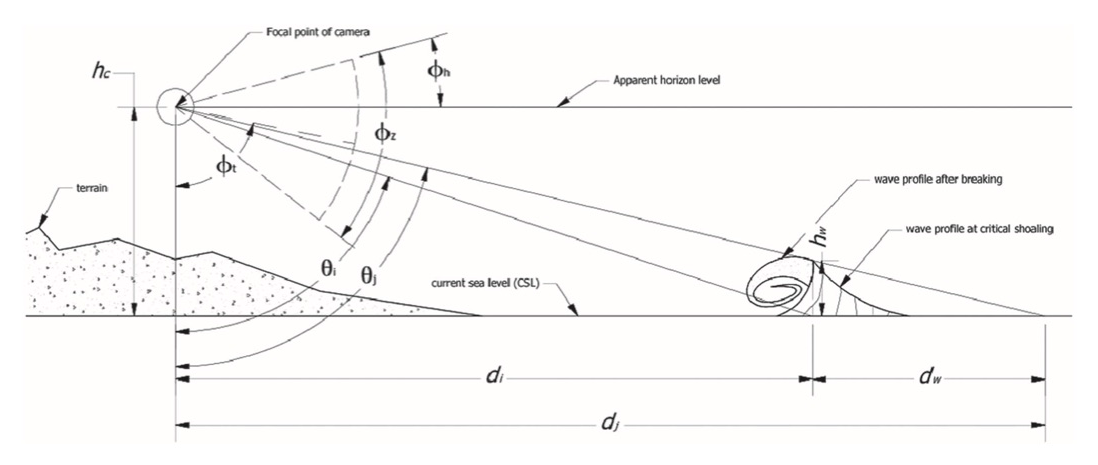
\includegraphics[scale=0.8]{beach_model_griffith.png}
  \caption[\small{Modelo Geométrico de uma Praia e Câmera. Fonte: Griffith University \cite{Griffith14}.}]{\label{FigBeachModel} \small{Modelo Geométrico de uma Praia e Câmera. Fonte: Griffith University \cite{Griffith14}.}}
\end{center}
\end{figure}
\paragraph{}A altura real de uma onda na imagem pode ser calculada pela equação:
\[
        h_{w} = h_{c}\Bigg(1 - \frac{tan(\theta_{i})}{tan(\theta_{j})}\Bigg)
\]
\noindent{}Onde \(h_{w}\) é a altura real de uma onda, \(\theta_{i}\) é o ângulo calculado do ponto mais baixo de uma onda e \(\theta_{j}\) é o ponto mais alto de uma onda. Utilizando uma câmera com baixa distorção, é possível calcular o ângulo \(\theta_{k}\) de um pixel \((x,k)\) através da equação:
\[
        \theta_{k} = \phi_{t} - \frac{\phi_{z}}{2} + \frac{k\phi_{z}}{V}
\]
\noindent{}onde \(V\) é a altura da imagem em pixels. A vantagem deste modelo em relação ao modelo furo-de-agulha é ser não só mais preciso, mas não depender da distância da câmera até a onda (valor $z$ do Modelo de Câmera Furo-de-Agulha), que pode ser altamente variável.

